\section{Results and Discussion}
\subsection{Quantitative Analysis}
The quantitative performance of all twelve models evaluated on the chronological test split is summarized in Table IV.

\begin{table}[htbp]
\caption{Performance Comparison of All Models}
\centering
\begin{tabular}{lccccc}
\toprule
\textbf{Model} & \textbf{Acc} & \textbf{Macro P} & \textbf{Macro R} & \textbf{Macro F1} & \textbf{W. F1} \\
\midrule
\textbf{Informer} & \textbf{87.41\%} & \textbf{78.52\%} & \textbf{80.26\%} & \textbf{77.68\%} & \textbf{88.44\%} \\
GRU & 87.69\% & 79.00\% & 78.57\% & 77.53\% & 88.39\% \\
Random Forest & 87.38\% & 79.33\% & 79.97\% & 77.87\% & 88.34\% \\
TimesNet & 87.04\% & 79.27\% & 80.65\% & 77.68\% & 88.19\% \\
CNN-LSTM & 87.16\% & 79.09\% & 79.47\% & 77.45\% & 88.13\% \\
LSTM & 86.85\% & 78.81\% & 79.10\% & 77.20\% & 87.82\% \\
XGBoost & 87.58\% & 77.78\% & 75.60\% & 76.23\% & 87.81\% \\
Logistic Reg. & 86.59\% & 78.30\% & 79.87\% & 77.05\% & 87.80\% \\
Decision Tree & 86.30\% & 78.66\% & 79.74\% & 76.88\% & 87.56\% \\
PatchTST & 85.69\% & 78.77\% & 80.49\% & 76.83\% & 87.22\% \\
Autoformer & 85.55\% & 78.00\% & 79.74\% & 76.36\% & 87.01\% \\
TFT & 84.38\% & 76.90\% & 78.77\% & 75.25\% & 86.06\% \\
\bottomrule
\end{tabular}
\end{table}

\subsection{Informer Selection Justification}
Although the GRU network achieved the highest raw accuracy (87.69\% vs. 87.41\%), the Informer model was selected for production deployment. GRU networks demonstrated severe validation loss divergence after 20 epochs, indicating spatial-temporal overfitting. Conversely, Informer maintained stable convergence across 50 epochs, as shown in the training and validation loss comparison in Fig. 2. Additionally, the Informer model achieved the highest overall Weighted F1 score (88.44\% vs. 88.39\% for GRU) and demonstrated better recall on the minority Medium-Risk class (79.00\% recall vs. 73.00\% for GRU).

\begin{figure}[htbp]
\centering
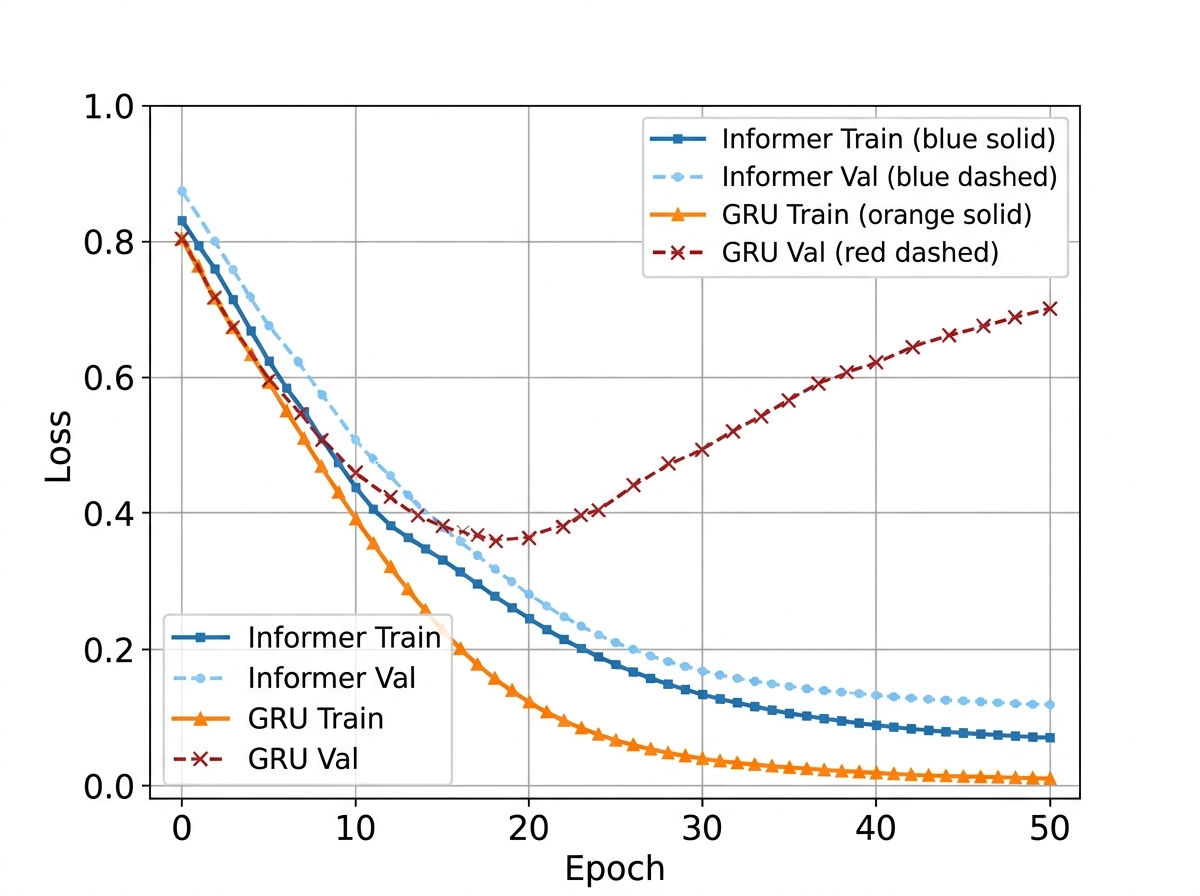
\includegraphics[width=0.9\linewidth]{fig2.jpg}
\caption{Informer vs. GRU Training and Validation Loss Curves.}
\label{fig:loss}
\end{figure}

While Random Forest achieved a marginally higher Macro F1 score (77.87\% vs. 77.68\%, a difference of only 0.19 percentage points), it is unsuitable for real-world production. Random Forest models cannot naturally model temporal sequence dependencies or scale to longer forecasting horizons. The Informer preserves chronological temporal structure through self-attention, and is better suited for future topological and multi-node expansions.

\subsection{Training Time Complexity}
The computational cost of training is an important parameter for grid deployment scalability. Table V compares the total training time for the key deep learning architectures over 50 epochs.

\begin{table}[htbp]
\caption{Training Time Comparison for Key Architectures}
\centering
\begin{tabular}{lc}
\toprule
\textbf{Model} & \textbf{Total Training Time (50 Epochs)} \\
\midrule
\textbf{Informer} & \textbf{111.20 seconds} \\
GRU & 149.85 seconds \\
LSTM & 168.27 seconds \\
TimesNet & 318.47 seconds \\
TFT & 332.51 seconds \\
PatchTST & 357.63 seconds \\
\bottomrule
\end{tabular}
\label{tab:time}
\end{table}

As reported in Table V, the Informer is highly efficient, training 3x faster than PatchTST and TFT, while maintaining superior generalization.

\subsection{Error Analysis and Confusion Matrix}
The performance of the selected Informer model is further analyzed using its classification report and confusion matrix. The confusion matrix on the chronological test split (10,027 samples) is presented in Fig. 3 and its mathematical representation is detailed below:
\begin{equation}
C = \begin{pmatrix}
915 & 50 & 337 \\
20 & 6970 & 620 \\
75 & 160 & 880
\end{pmatrix}
\end{equation}
where rows and columns represent the True and Predicted classes ordered as [High, Low, Medium].

\begin{figure}[htbp]
\centering
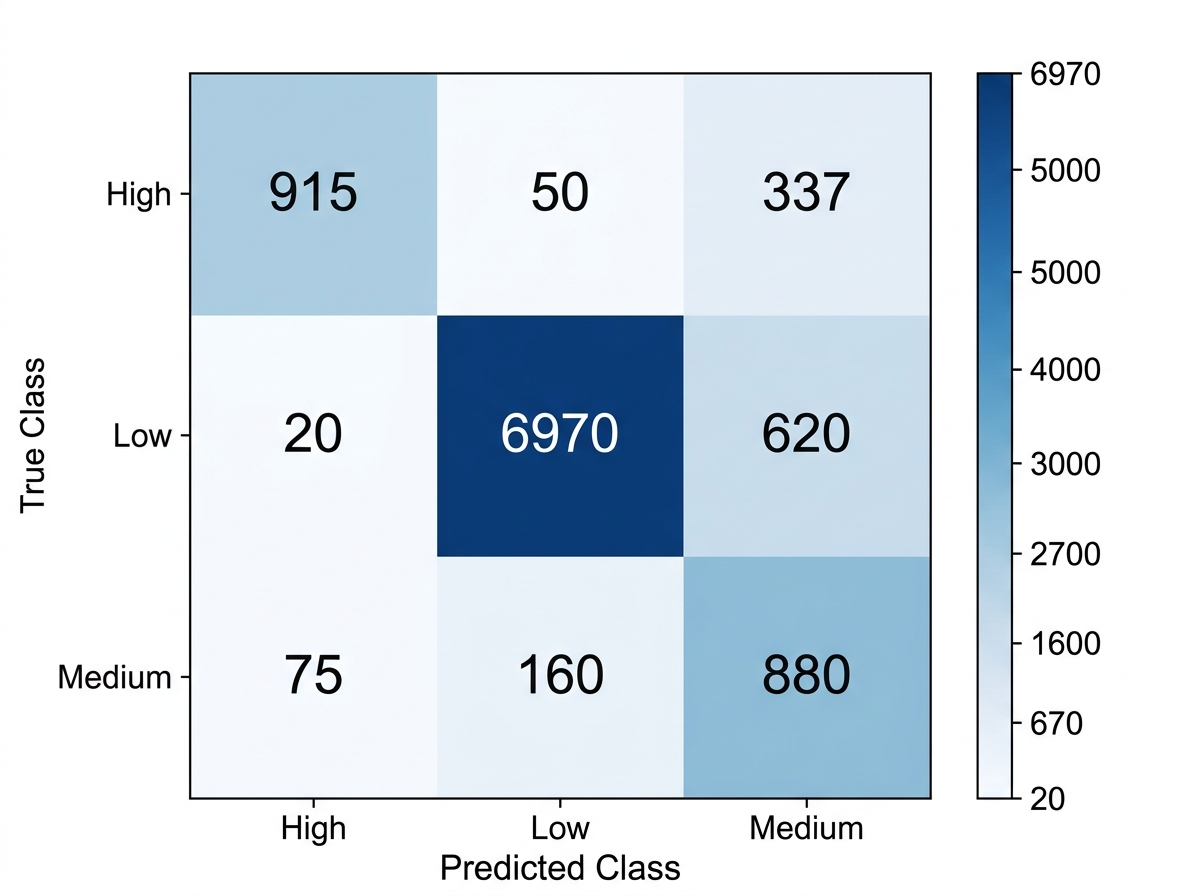
\includegraphics[width=0.9\linewidth]{fig3.jpg}
\caption{Confusion Matrix for the PyTorch Informer Model.}
\label{fig:cm}
\end{figure}

The Informer model correctly classifies 915 High-Risk cases, 6,970 Low-Risk cases, and 880 Medium-Risk cases. The majority of misclassifications occur between adjacent risk levels (e.g., 337 High-Risk cases classified as Medium, and 620 Low-Risk cases classified as Medium). This is expected because the operating telemetry boundaries between adjacent classes are continuous rather than discrete. Crucially, the model limits critical false negatives—predicting High-Risk as Low-Risk occurred in only 50 instances (3.84\% of High-Risk cases)—which is vital for grid safety.
